% !TEX root = ../main.tex

\documentclass[../../main.tex]{subfiles}
\begin{document}
\definecolor{qqccqq}{rgb}{0,0.8,0}
\definecolor{qqqqff}{rgb}{0,0,1}
\question \textbf{Ejercicio 1:} Demostrar que $\int\limits_{0}^b x^3 dx = \frac{b^4}{4}$ considerando particiones de $n$
subintervalos y usando la formula para $\sum\limits_{i=1}^n i^3$.
\begin{proof}
    Sea $P = \{x_0, x_1, \dots, x_n\}$ de forma que $x_i - x_{i-1} = \frac{b}{n}$ para todo $i$ entre $1$ y $n$. Observese entonces que $U(f, P)$ y $L(f, P)$ pueden ser escritos como:
    \begin{align*}
        U(f, P) &= \sum_{i = 1}^n M_i (x_i-x_{i-1}) & L(f, P) &= \sum_{i = 1}^n m_i (x_i - x_{i-1})\\
        &= \sum_{i = 1}^n x_i^3 \cdot \frac{b}{n} & &= \sum_{i=1}^n x_{i-1}^3 \cdot \frac{b}{n}\\
        &= \sum_{i = 1}^n \left(i \cdot \frac{b}{n}\right)^3 \cdot \frac{b}{n} & &= \sum_{j = 0}^{n-1} x_j^3 \cdot \frac{b}{n}\\
        &= \sum_{i = 1}^n i^3 \cdot \frac{b^3}{n^3} \cdot \frac{b}{n} & &= \sum_{j = 1}^{n-1} j^3 \cdot \frac{b^3}{n^3} \cdot \frac{b}{n}\\
        &= \frac{b^4}{n^4} \sum_{i = 1}^n i^3 & &= \frac{b^4}{n^4} \sum_{j = 1}^{n-1} j^3\\
        &= \frac{b^4}{n^4} \cdot \frac{n^2 \cdot (n+1)^2}{4} & &= \frac{b^4}{n^4} \cdot \frac{n^2 \cdot (n-1)^2}{4}\\
    \end{align*}

    Es fácil notar entonces que:

    $$L(f, P) < \frac{b^4}{n^4} < U(f, P)$$

    Y gracias a que $n$ puede hacerse tan grande como se desee, podemos hacer que $U(f, P) - L(f, P)$ sea tan pequeño como se desee, concluyendo entonces que al ser la integral el
    único número con dicha propiedad:
    $$\int_0^b x^3 dx = \frac{b^4}{4}$$
    De manera más general se puede llegar al resultado:
    \begin{align*}
        U(f, P) - L(f, P) &= \frac{b^4}{2 \cdot n}
    \end{align*}
    Lo que hace más evidente la afirmación anterior.
\end{proof}

\question \textbf{Ejercicio 2:} Demostrar de forma similar que $\int\limits_{0}^b x^4 dx = \frac{b^5}{5}$.
\begin{proof}
    Sea $P = \{x_0, x_1, \dots, x_n\}$ de forma que $x_i - x_{i-1} = \frac{b}{n}$ para todo $i$ entre $1$ y $n$. Observese entonces que $U(f, P)$ y $L(f, P)$ pueden ser escritos como:
    \begin{align*}
        U(f, P) &= \sum_{i = 1}^n M_i (x_i-x_{i-1}) & L(f, P) &= \sum_{i = 1}^n m_i (x_i - x_{i-1})\\
        &= \sum_{i = 1}^n x_i^4 \cdot \frac{b}{n} & &= \sum_{i=1}^n x_{i-1}^4 \cdot \frac{b}{n}\\
        &= \sum_{i = 1}^n \left(i \cdot \frac{b}{n}\right)^4 \cdot \frac{b}{n} & &= \sum_{j = 0}^{n-1} x_j^4 \cdot \frac{b}{n}\\
        &= \sum_{i = 1}^n i^4 \cdot \frac{b^4}{n^4} \cdot \frac{b}{n} & &= \sum_{j = 1}^{n-1} j^4 \cdot \frac{b^4}{n^4} \cdot \frac{b}{n}\\
        &= \frac{b^5}{n^5} \sum_{i = 1}^n i^4 & &= \frac{b^5}{n^5} \sum_{j = 1}^{n-1} j^4\\
        &= \frac{b^5}{n^5} \cdot \frac{n  (n+1) (2n+1) (3n^2+3n-1)}{30} & &= \frac{b^5}{n^5} \cdot \frac{n  (n-1)  (2n-1) (3n^2-3n-1)}{30}\\
    \end{align*}

    Es fácil notar entonces que:

    $$L(f, P) < \frac{b^5}{n^5} < U(f, P)$$

    Y gracias a que $n$ puede hacerse tan grande como se desee, podemos hacer que $U(f, P) - L(f, P)$ sea tan pequeño como se desee, concluyendo entonces que al ser la integral el
    único número con dicha propiedad:
    $$\int_0^b x^4 dx = \frac{b^5}{5}$$

    De manera más general se puede llegar al resultado:
    \begin{align*}
        U(f, P) - L(f, P) &= \frac{b^5}{n}
    \end{align*}
    Lo que hace más evidente la afirmación anterior.
\end{proof}

\question \textbf{Ejercicio 5:} Evaluar sin hacer calculos:
\begin{partes}
\parte $\int_{-1}^1 x^3 \cdot \sqrt{1-x^2}dx$\\

Para empezar, determinaremos el comportamiento de la función con respecto a paridad:
\begin{align*}
    f(-x) &= (-x)^3 \cdot \sqrt{1-(-x)^2}\\
    &= -(x^3) \cdot \sqrt{1-x^2}\\
    &= -f(x)
\end{align*}
Por lo que concluimos que $f$ es una función impar. Luego, eso quiere decir que:
\begin{align*}
    \int_{-1}^1 x^3 \cdot \sqrt{1-x^2}dx &= 0
\end{align*}

\parte $\int_{-1}^1 (x^5+3) \cdot \sqrt{1-x^2}dx$
Empecemos por despejar la función como procede:
\begin{align*}
    \int_{-1}^1 (x^5+3) \cdot \sqrt{1-x^2}dx &= \int_{-1}^1 x^5 \cdot \sqrt{1-x^2} + 3\cdot\sqrt{1-x^2}dx\\
    &= \int_{-1}^1 x^5 \cdot \sqrt{1-x^2} dx +\int_{-1}^1 3\cdot\sqrt{1-x^2}dx\\
\end{align*}
Luego, gracias a que la función $x^5 \cdot \sqrt{1-x^2}$ es impar, la integral de dicha función entre $-1$ y $1$ será 0. Solo se debe hallar el valor de:
\begin{align*}
    \int_{-1}^1 3\cdot\sqrt{1-x^2}dx &= 3\int_{-1}^1 \sqrt{1-x^2}
\end{align*}
Y dado que la función es par, solo es necesario conocer el valor de:
\begin{align*}
    2 \cdot \int_{0}^1 \sqrt{1-x^2}
\end{align*}
Pero dicha area será la cuarta parte del área de una circunferencia de radio $1$. Lo que sería:
\begin{align*}
    \frac{A}{4} &= \frac{\pi \cdot r^2}{4}\\
    &= \frac{\pi}{4}
\end{align*}
Luego, eso significa que:
\begin{align*}
    2 \cdot \int_{0}^1 \sqrt{1-x^2} &= \frac{\pi}{2}
\end{align*}
Y entonces:
\begin{align*}
    3\int_{-1}^1 \sqrt{1-x^2} &= \frac{3\pi}{2}
\end{align*}
Siendo el anterior resultado, el correspondiente a la integral original.

\end{partes}

\question \textbf{Ejercicio 7:} Decidir cuales de las siguientes funciones son integrables en $[0, 2]$ y cálcular la integral cuando sea posible.
\begin{partes}
    \parte $f(x) = \begin{cases}
        x, & 0\le x < 1\\
        x-2, & 1\le x \le 2\\
    \end{cases}$\\
    \begin{proof}
        Sea $\epsilon > 0$, queremos determinar una partición $P_\epsilon$ de modo que:
        $$U(f, P_\epsilon) - L(f, P_\epsilon) < \epsilon$$
        Para ejercicios practicos, es conveniente hacer que $1 \in P_\epsilon$ de forma que para algún $k$ se tendrá que $x_k = 1$.Definamos entonces cada uno de los terminos:
        \begin{align*}
            U(f, P) &= \sum_{i = 1}^n M_i(x_i - x_{i-1})\\
            &= \sum_{i = 1}^{k} M_i(x_i - x_{i-1}) + \sum_{i = k+1}^n M_i(x_i - x_{i-1})\\
            &= \sum_{i = 1}^{k} x_i(x_i - x_{i-1}) + 1 + \sum_{i = k+2}^n (x_i-2)(x_i - x_{i-1})\\ 
        \end{align*}
        \begin{align*}
            L(f, P) &= \sum_{i = 1}^n m_i(x_i - x_{i-1})\\
            &= \sum_{i = 1}^{k} m_i(x_i - x_{i-1}) + \sum_{i = k+1}^{n} m_i(x_i - x_{i-1})\\
            &= \sum_{i = 1}^{k-1} x_{i-1}(x_i - x_{i-1}) + (-1) + \sum_{i = k+1}^{n} (x_{i-1}-2)(x_i - x_{i-1})
        \end{align*}
    \end{proof}

    \parte $f(x) = \begin{cases}
        x, & 0\le x \le 1\\
        x-2, & 1< x \le 2\\
    \end{cases}$

    \parte $f(x) = x + [x]$

    \parte $f(x) = \begin{cases}
        x + [x],& x \text{ rational}\\
        0,& x \text{ irrational}\\
    \end{cases}$

    \parte $f(x) = \begin{cases}
        1,& x \text{ es de la forma $a+b\sqrt{2}$ para $a, b \in \mathbb{Q}$}\\
        0,& x \text{ no es de dicha forma}\\
    \end{cases}$

    \parte $f(x) = \begin{cases}
        \frac{1}{\left[\frac{1}{x}\right]},&  0 < x \le 1\\
        0,& x = 0 \text{ or } x > 1\\
    \end{cases}$
\end{partes}

\question \textbf{Ejercicio 8:} Encontrar el area de las regiones delimitadas por:
\begin{partes}
    \parte Las gráficas de $f(x) = x^2$ y $g(x) = \frac{x^2}{2}+2$\\
    \begin{center}
        \begin{figure}[h]
            \centering
            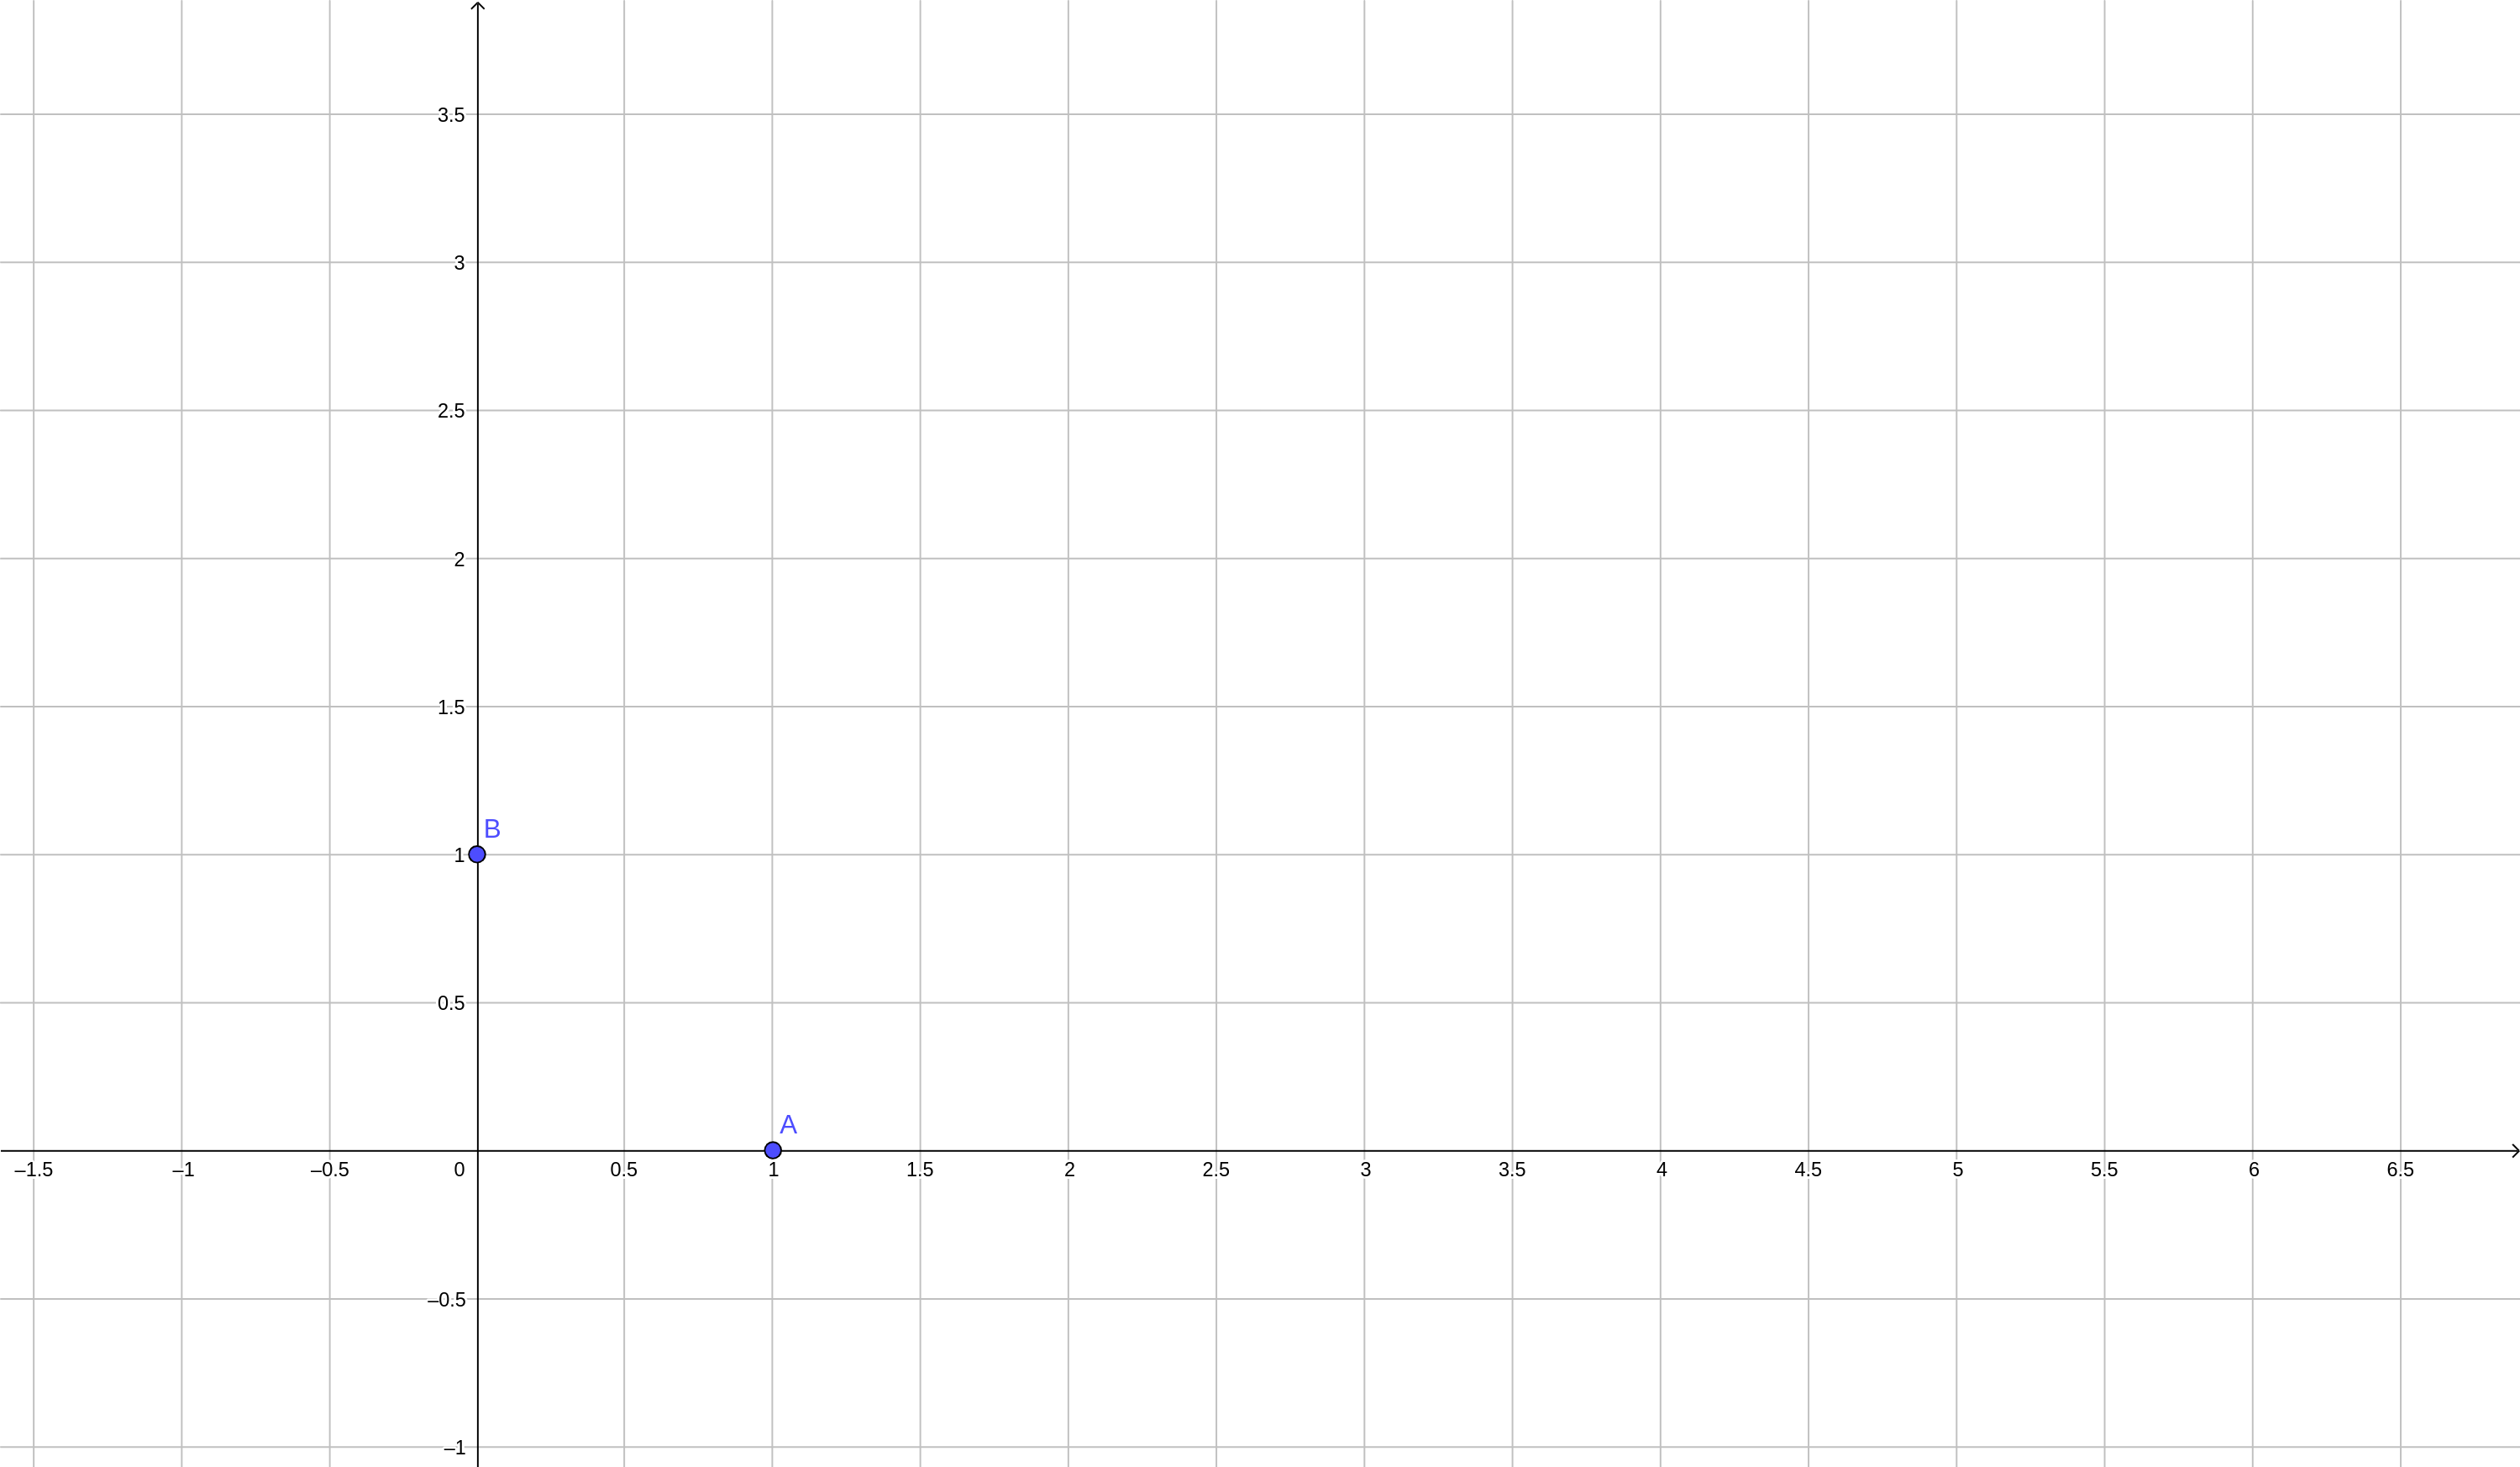
\includegraphics{Parte 1/grafica1.png}
        \end{figure}        
    \end{center}

    En este caso, bastará con calcular la integral de ambas funciones en el intervalo $[-2, 2]$, siendo el intervalo donde
    ambas funciones delimitan un area especifica. Luego, dado que en dicho intervalo se tiene la desigualdad $g(x) \ge f(x)$,
    el area de la región delimitada será el area bajo la curva de $g$ sin el area bajo la curva de $f$. Esto es:
    \begin{align*}
        \int_{-2}^2 g(x)-f(x) dx &= \int_{-2}^2 g(x)dx - \int_{-2}^2 f(x)dx\\
        &= \int_{-2}^2 \frac{x^2}{2}+2 dx- \int_{-2}^2 x^2dx\\
        &= \frac{1}{2}\int_{-2}^2 x^2dx + \int_{-2}^2 2dx - \int_{-2}^2 x^2dx\\
        &= \frac{1}{2} \cdot 2 \cdot \frac{8}{3} + 8 - 2 \cdot \frac{8}{3}\\
        &= \frac{16}{3}
    \end{align*}
    Por lo que el área delimitada por dichas graficas será $\frac{16}{3}$ unidades.

    \parte Las gráficas de $f(x) = x^2$, $g(x) = -x^2$ y las lineas verticales que pasan por $(-1, 0)$ y $(1, 0)$\\
    \begin{figure}[h]
        \centering
        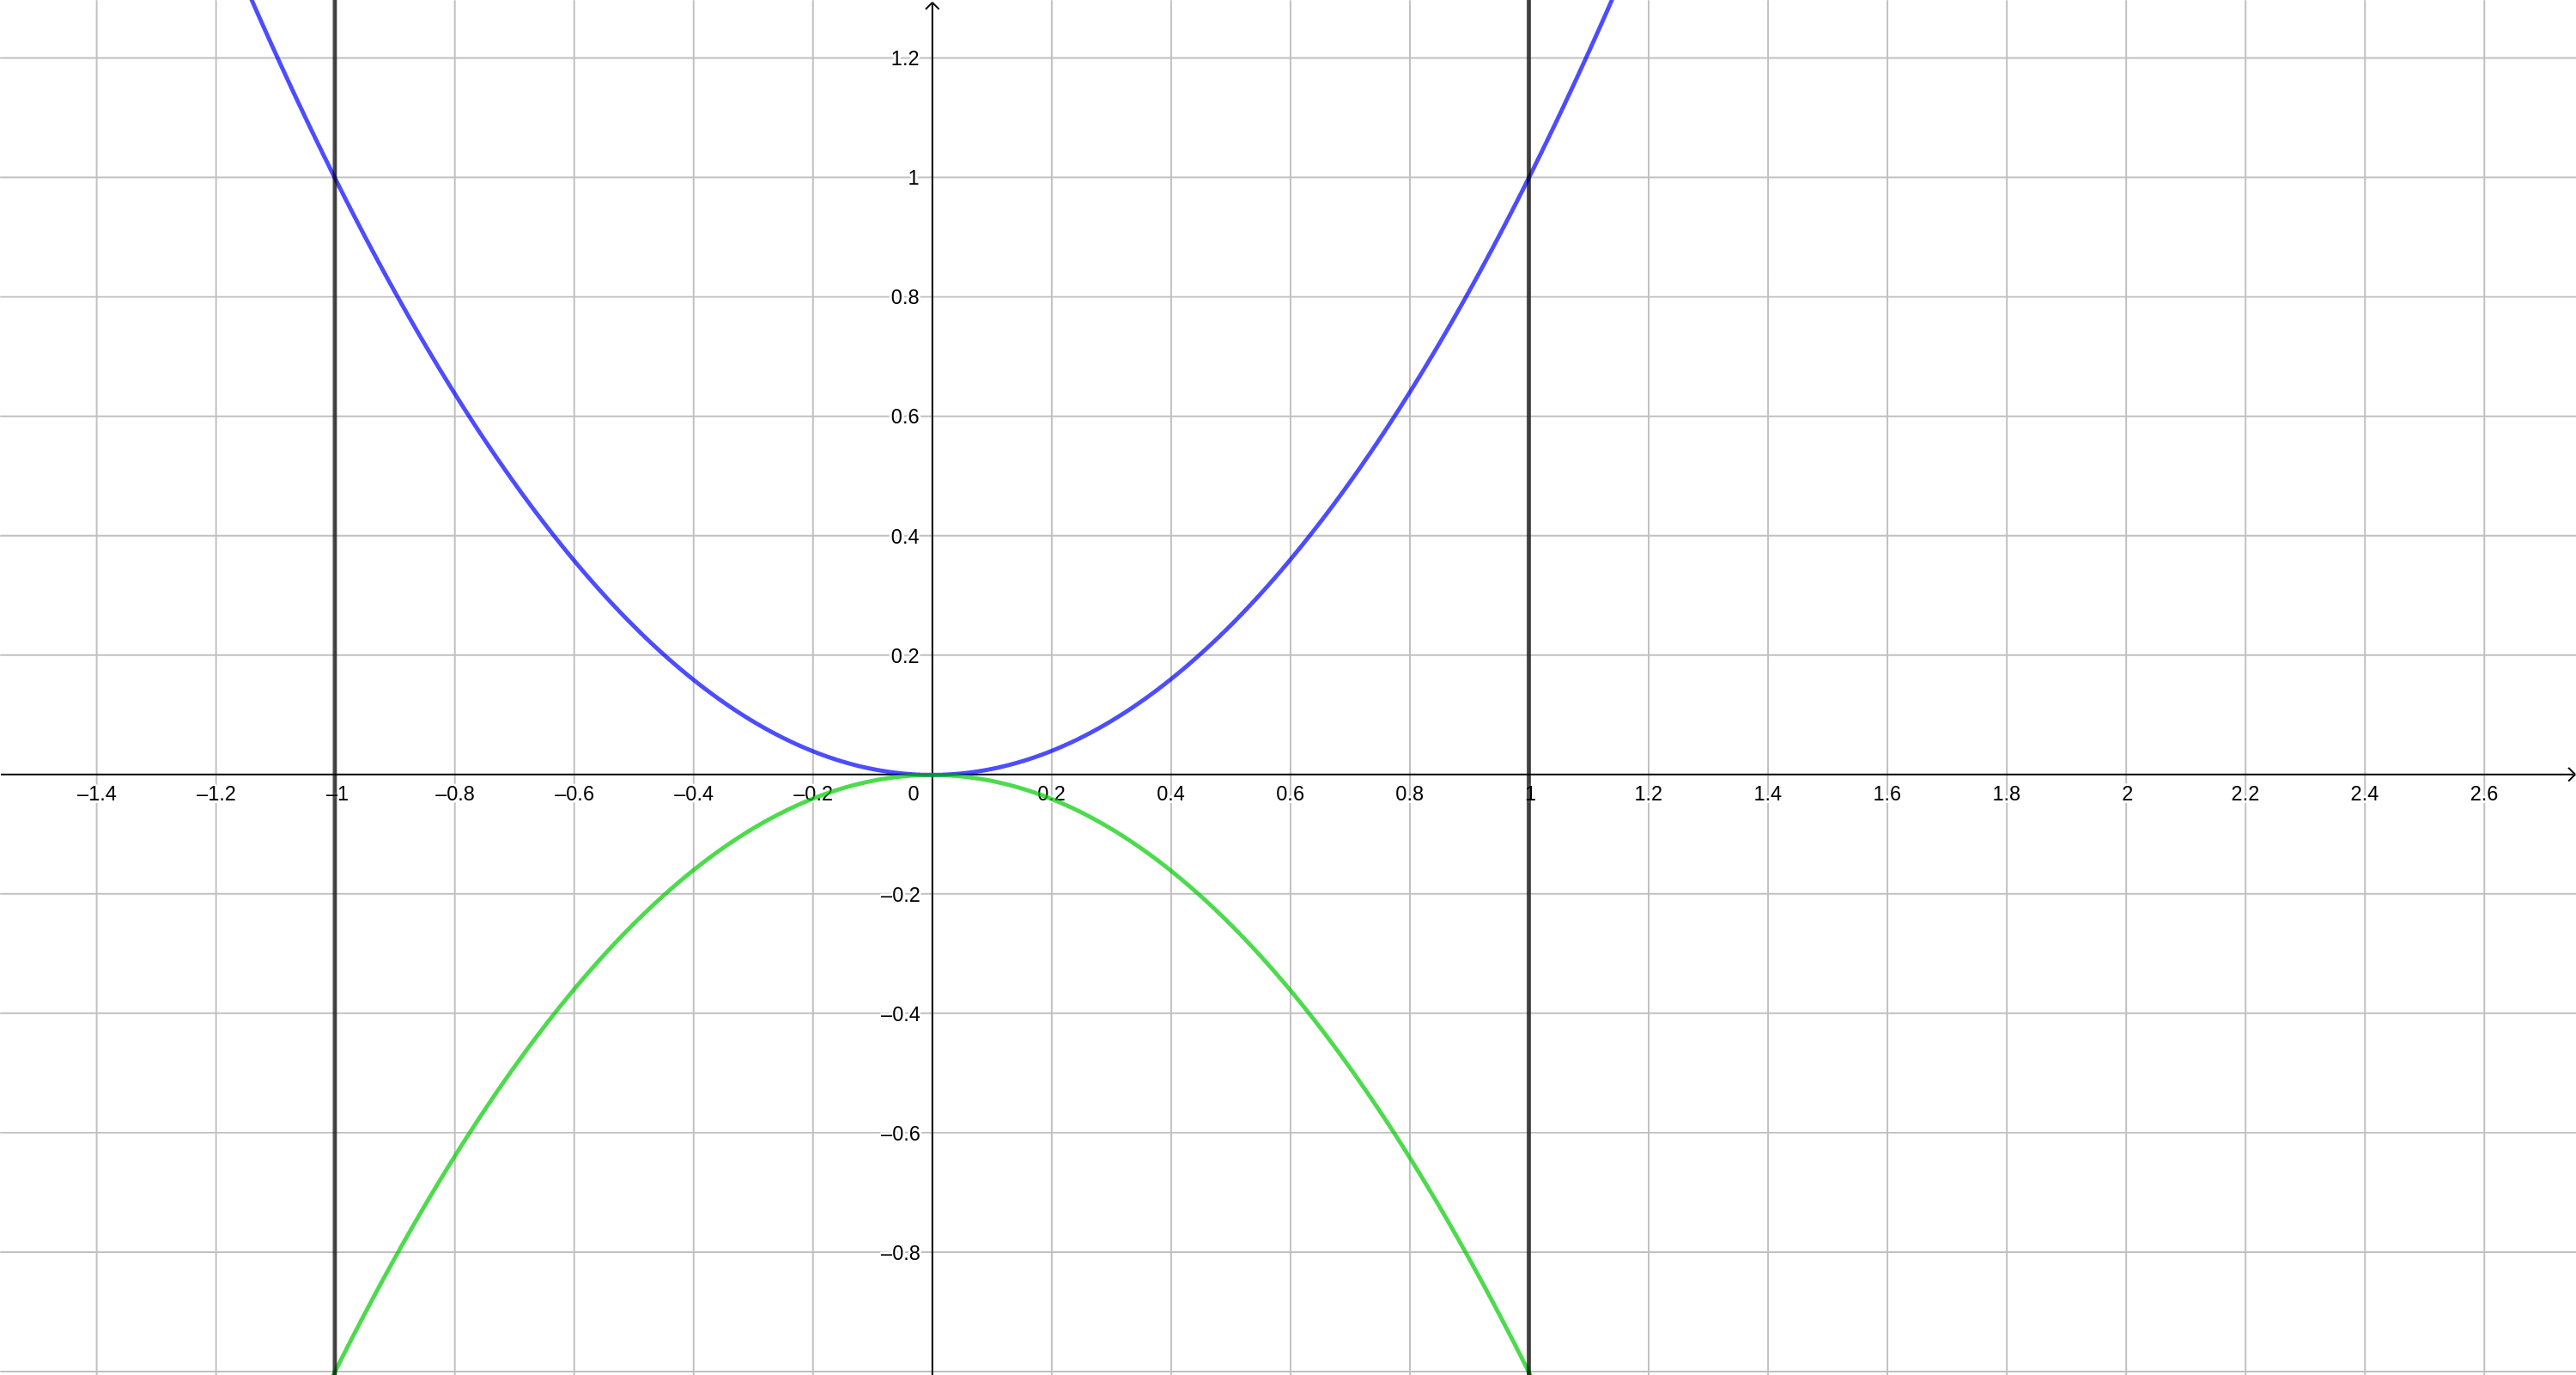
\includegraphics[width=12cm]{Parte 1/grafica2.png}
    \end{figure}
    Notese que la función $f$ es un reflejo de la función $g$ sobre el eje $x$, por lo que bastará con cálcular el area de la región delimitada por
    encima del eje $x$ para determinar el area total. Además, note que las dos rectas verticales intersecan a la función $f$ en los puntos $(-1, 1)$ y $(1, 1)$. Esto
    permite delimitar el problema a calcular el area bajo la curva de la función $f$ en el intervalo $[-1, 1]$.
    \begin{align*}
        \int_{-1}^1 f(x) dx &= \int_{-1}^1 x^2 dx\\
        &= \frac{1^3}{3} - \frac{(-1)^3}{3}\\
        &= \frac{1}{3} + \frac{1}{3}\\
        &= \frac{2}{3}\\
    \end{align*}
    Luego, el area total de la región delimitada por las dos funciones y las dos rectas será el doble del area anterior, es decir,
    $\frac{4}{3}$ unidades.

    \parte Las gráficas de $f(x) = x^2$ y $g(x) = 1-x^2$
    \begin{figure}[h]
        \centering
        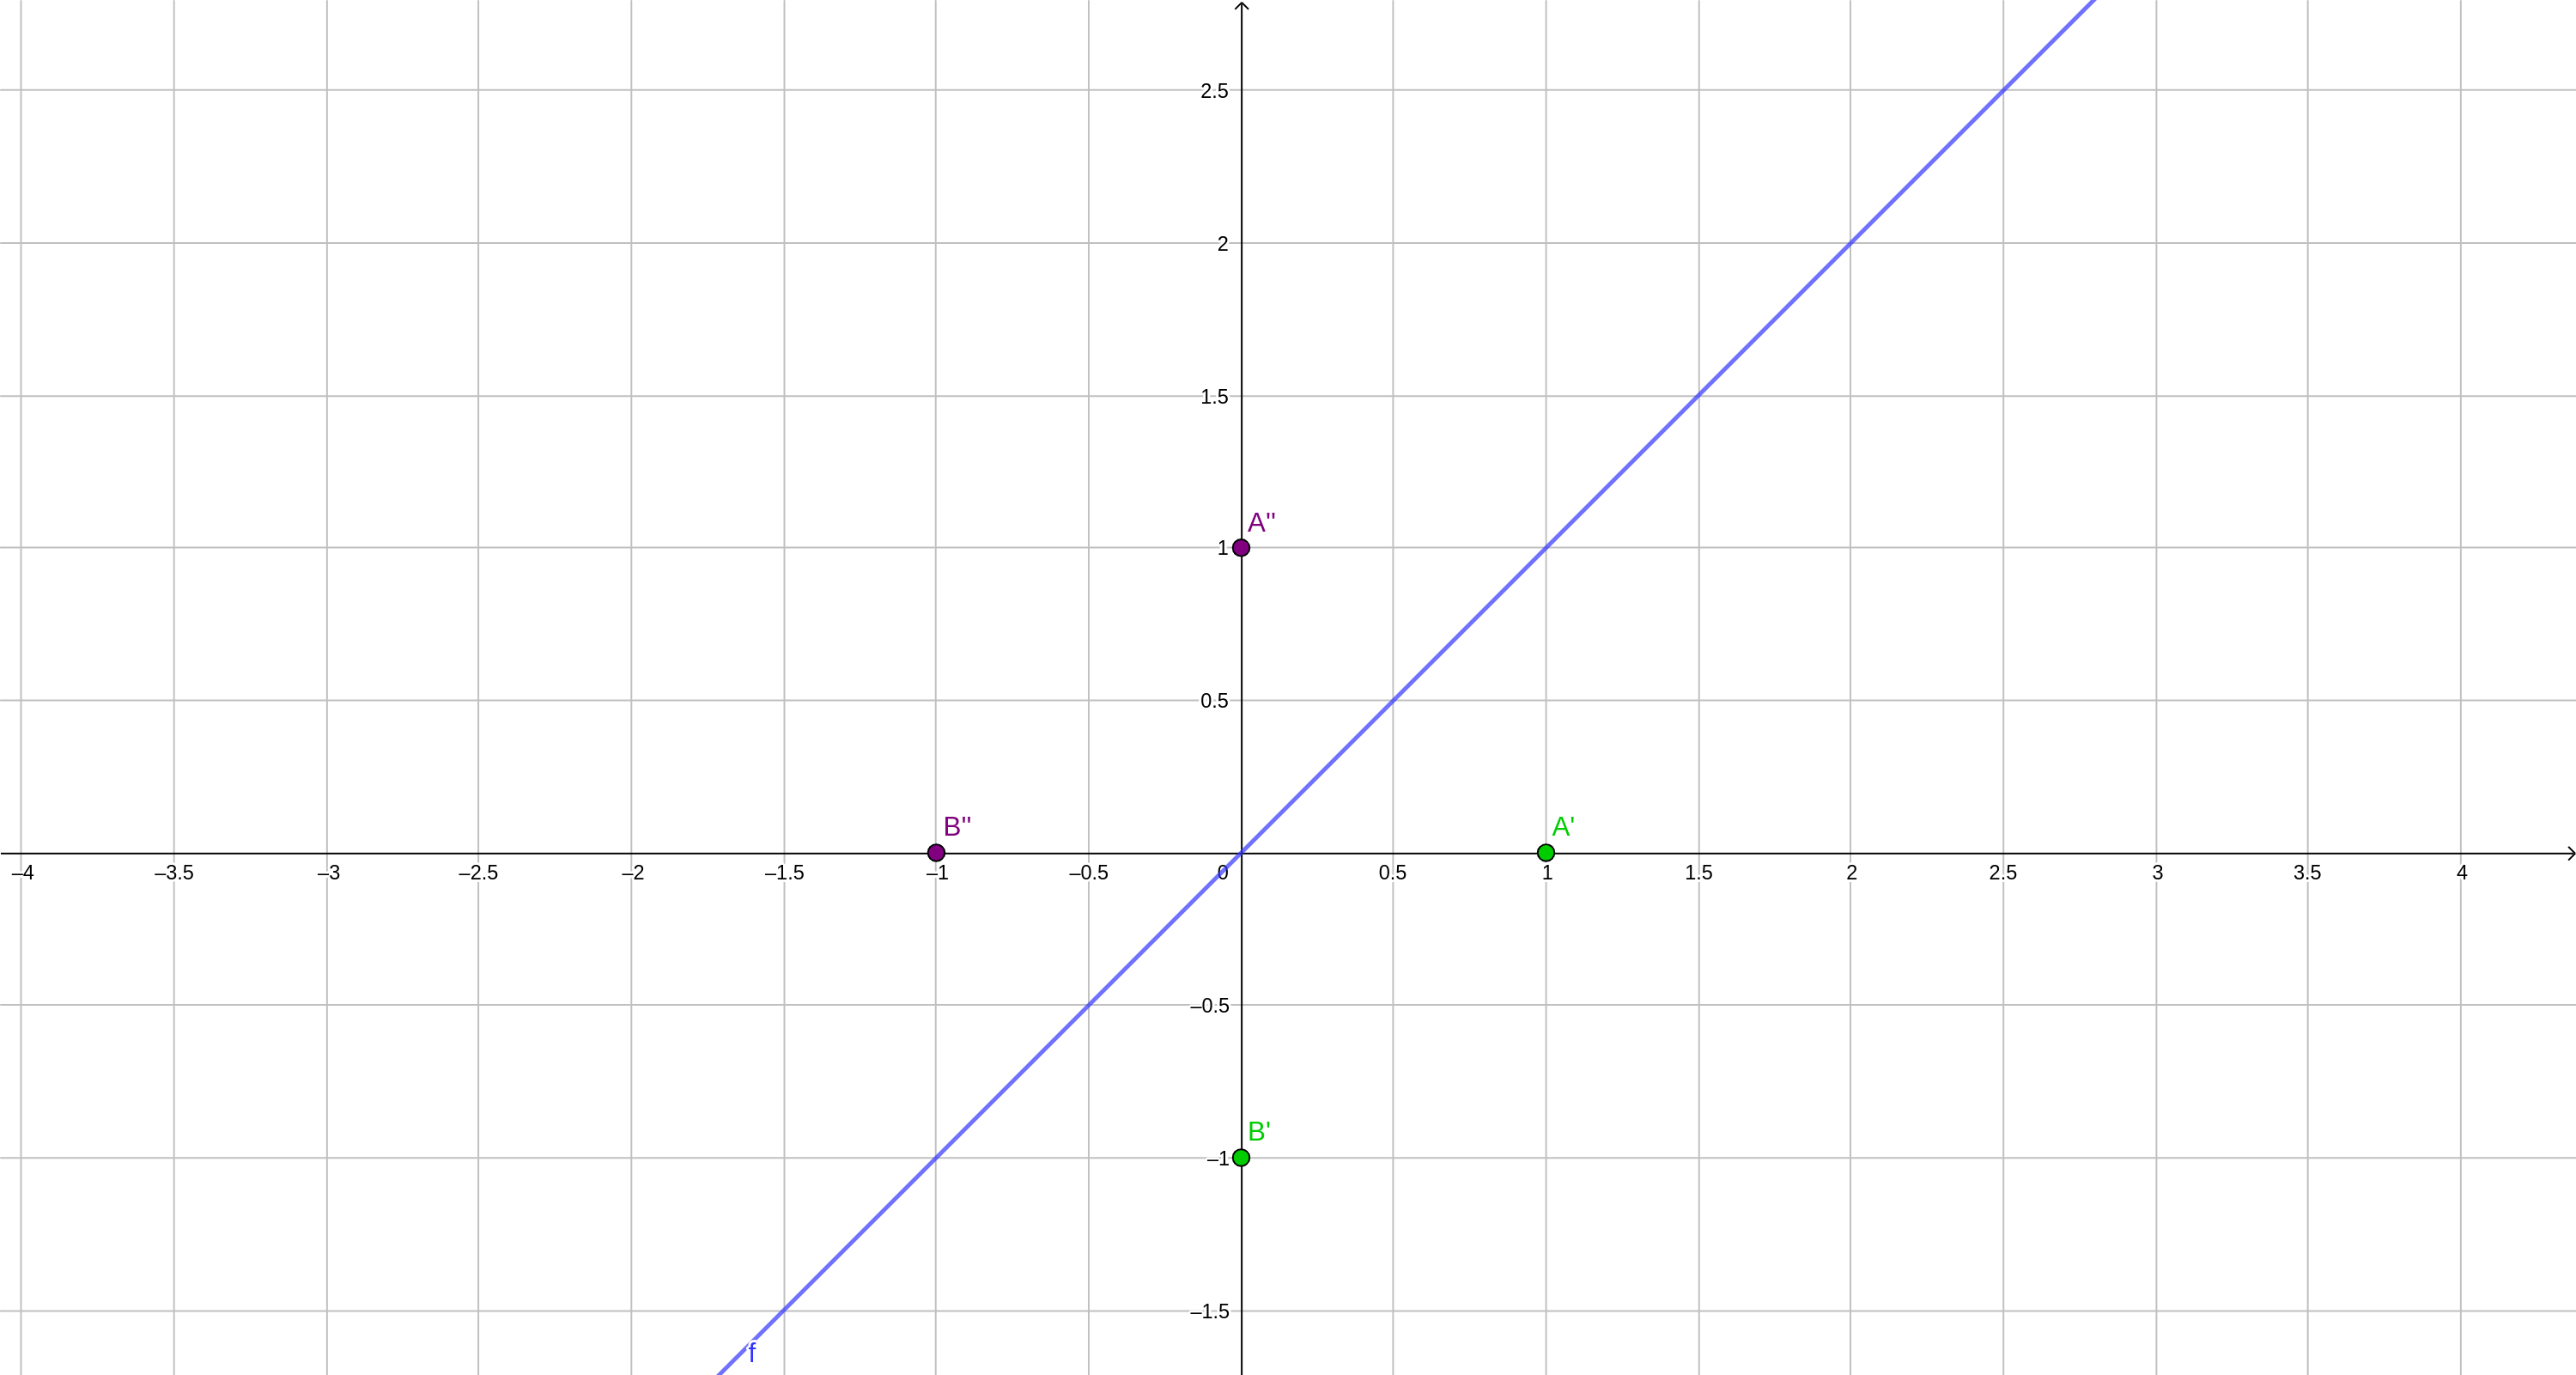
\includegraphics[width=12cm]{Parte 1/grafica3.png}
    \end{figure} 
    La figura determinada por dichas funciones se refleja sobre el eje $y$ al ser ambas funciones pares. Por lo que es suficiente encontrar
    el area de un lado de la gráfica. Determinando primero las restricciones de las funciones:
    \begin{align*}
        x^2 &= 1-x^2\\
        2x^2 &= 1\\
        x^2 &= \frac{1}{2}\\
        x &= \pm \sqrt{\frac{1}{2}}\\
    \end{align*}
    Con esto en mente, la integral necesaria para determinar el area es aquella del intervalo $[0, \frac{\sqrt{2}}{2}]$ teniendo en cuenta que la función
    $g$ es mayor a la función $f$ en los valores de este intervalo. Por lo que el area de la figura será:
    \begin{align*}
        \int_{0}^{\frac{\sqrt{2}}{2}} 1- x^2 - x^2 dx &= \int_{0}^{\frac{\sqrt{2}}{2}} 1-2x^2 dx\\
        &= \int_{0}^{\frac{\sqrt{2}}{2}} 1 \cdot dx - 2\int_{0}^{\frac{\sqrt{2}}{2}} x^2 dx\\  
        &= \frac{\sqrt{2}}{2} - 2 \cdot \left(\frac{\left(\frac{\sqrt{2}}{2}\right)^3}{3}\right)\\
        &= \frac{\sqrt{2}}{2} - 2 \cdot \left(\frac{\frac{2\sqrt{2}}{8}}{3}\right)\\
        &= \frac{\sqrt{2}}{2} - \frac{\frac{2\sqrt{2}}{4}}{3}\\
        &= \frac{\sqrt{2}}{2} - \frac{2\sqrt{2}}{12}\\
        &= \frac{\sqrt{2}}{2} \cdot \left(1 - \frac{2}{6}\right)\\
        &= \frac{\sqrt{2}}{2} \cdot \left(1 - \frac{1}{3}\right)\\
        &= \frac{\sqrt{2}}{2} \cdot \frac{2}{3}\\
        &= \frac{\sqrt{2}}{3}
    \end{align*}
    Por lo que el área de la figura completa será $\frac{2\sqrt{2}}{3}$ unidades.\\

    \parte Las gráficas de $f(x) = x^2$, $g(x) = 1-x^2$ y $h(x) = 2$\\
    \begin{figure}[h]
        \centering
        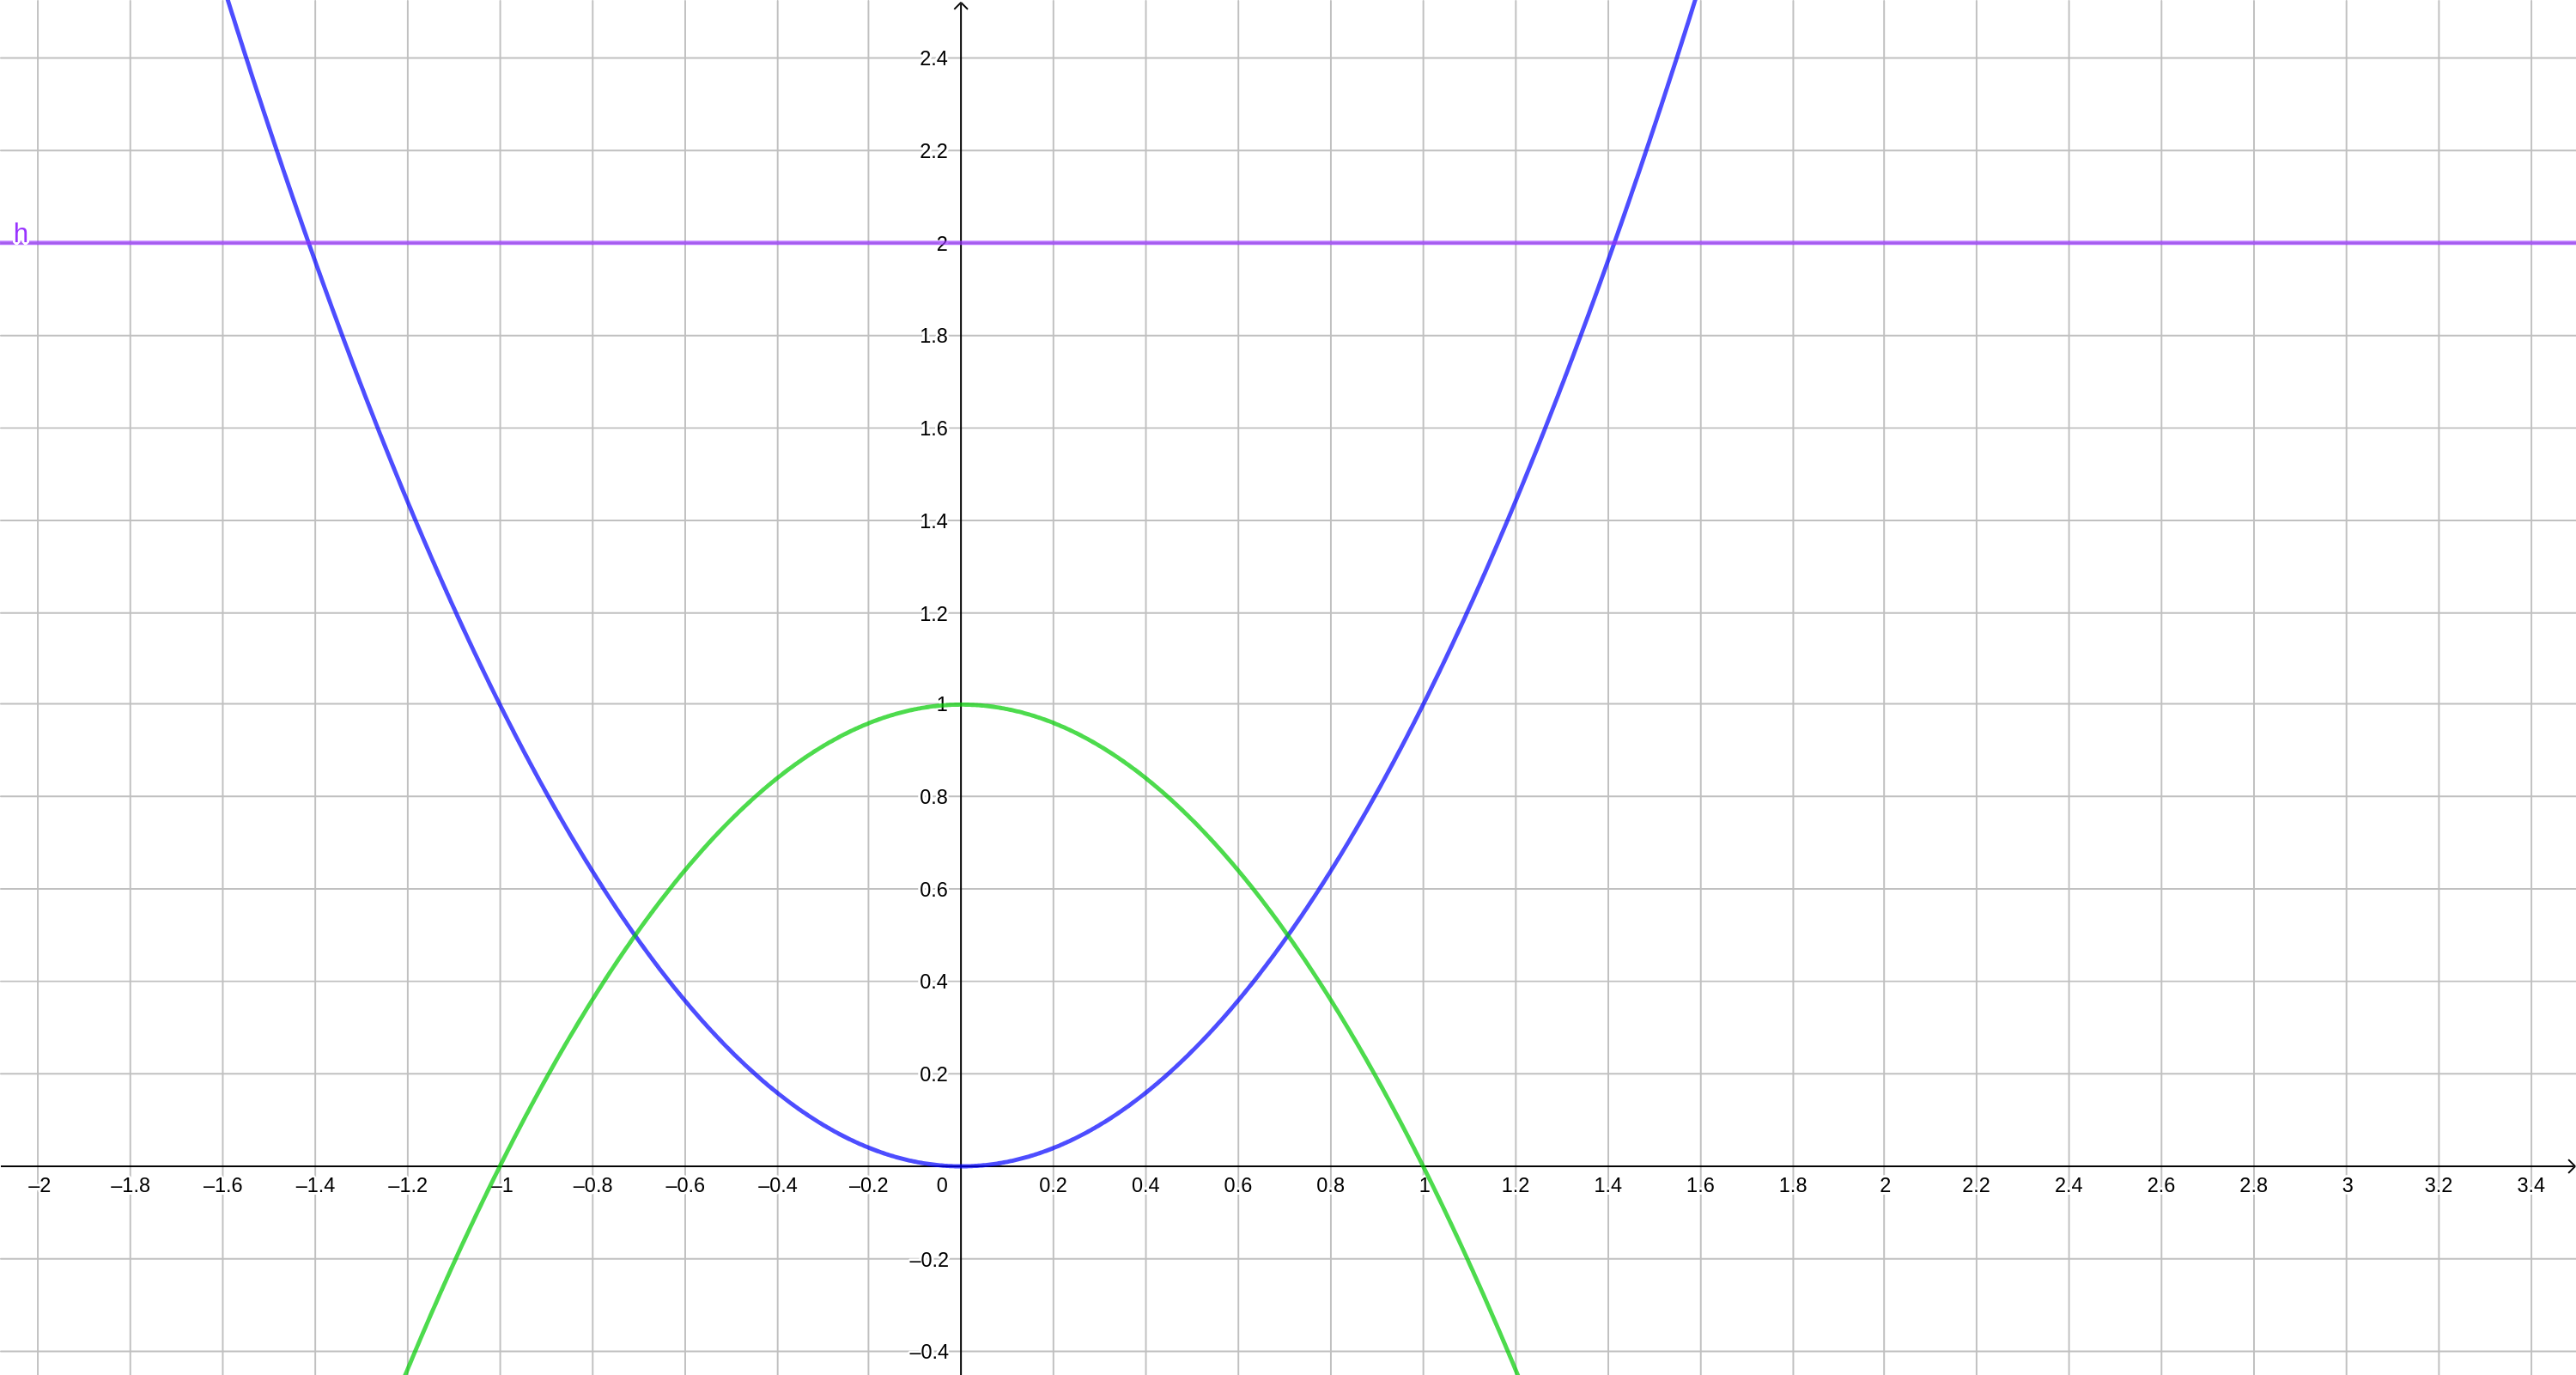
\includegraphics[width=12cm]{Parte 1/grafica4.png}
    \end{figure}
    En este caso, es importante notar que la región delimitada por las tres figuras tiene que estar por encima del eje $x$ y por debajo de
    $y=2$. Dado que $h$ interseca a $f$ en los puntos $\sqrt{2}$ y $-\sqrt{2}$, el area de la región entre $f$ y $h$ será expresada como sigue:
    \begin{align*}
        \int_{0}^{\sqrt{2}} 2-x^2 &= \int_{0}^{\sqrt{2}} 2 dx- \int_{0}^{\sqrt{2}} x^2 dx\\
        &= 2 \cdot \sqrt{2} - \frac{2\sqrt{2}}{3}\\
        &= 2\cdot \sqrt{2} \cdot \left(1 - \frac{1}{3}\right)\\
        &= 2\cdot \sqrt{2} \cdot \frac{2}{3}\\
        &= \frac{4\sqrt{2}}{3}
    \end{align*}
    Por lo que el area entre $f$ y $h$ será $\frac{8\sqrt{2}}{3}$. Luego, para obtener el area deseada sustraemos el area entre $f$ y $h$ del area
    entre $f$ y $g$ que fue determinada en el problema anterior.
    \begin{align*}
        \frac{8\sqrt{2}}{3} - \frac{2\sqrt{2}}{3} &= \frac{8\sqrt{2} - 2\sqrt{2}}{3}\\
        &= \frac{6\sqrt{2}}{3}
    \end{align*}
    Por lo que el area delimitada por las tres gráficas será $\frac{6\sqrt{2}}{3}$.

    \parte Las gráficas de $f(x) = x^2$, $g(x) = x^2-2x+4$ y el eje vertical\\
    \begin{figure}[h]
        \centering
        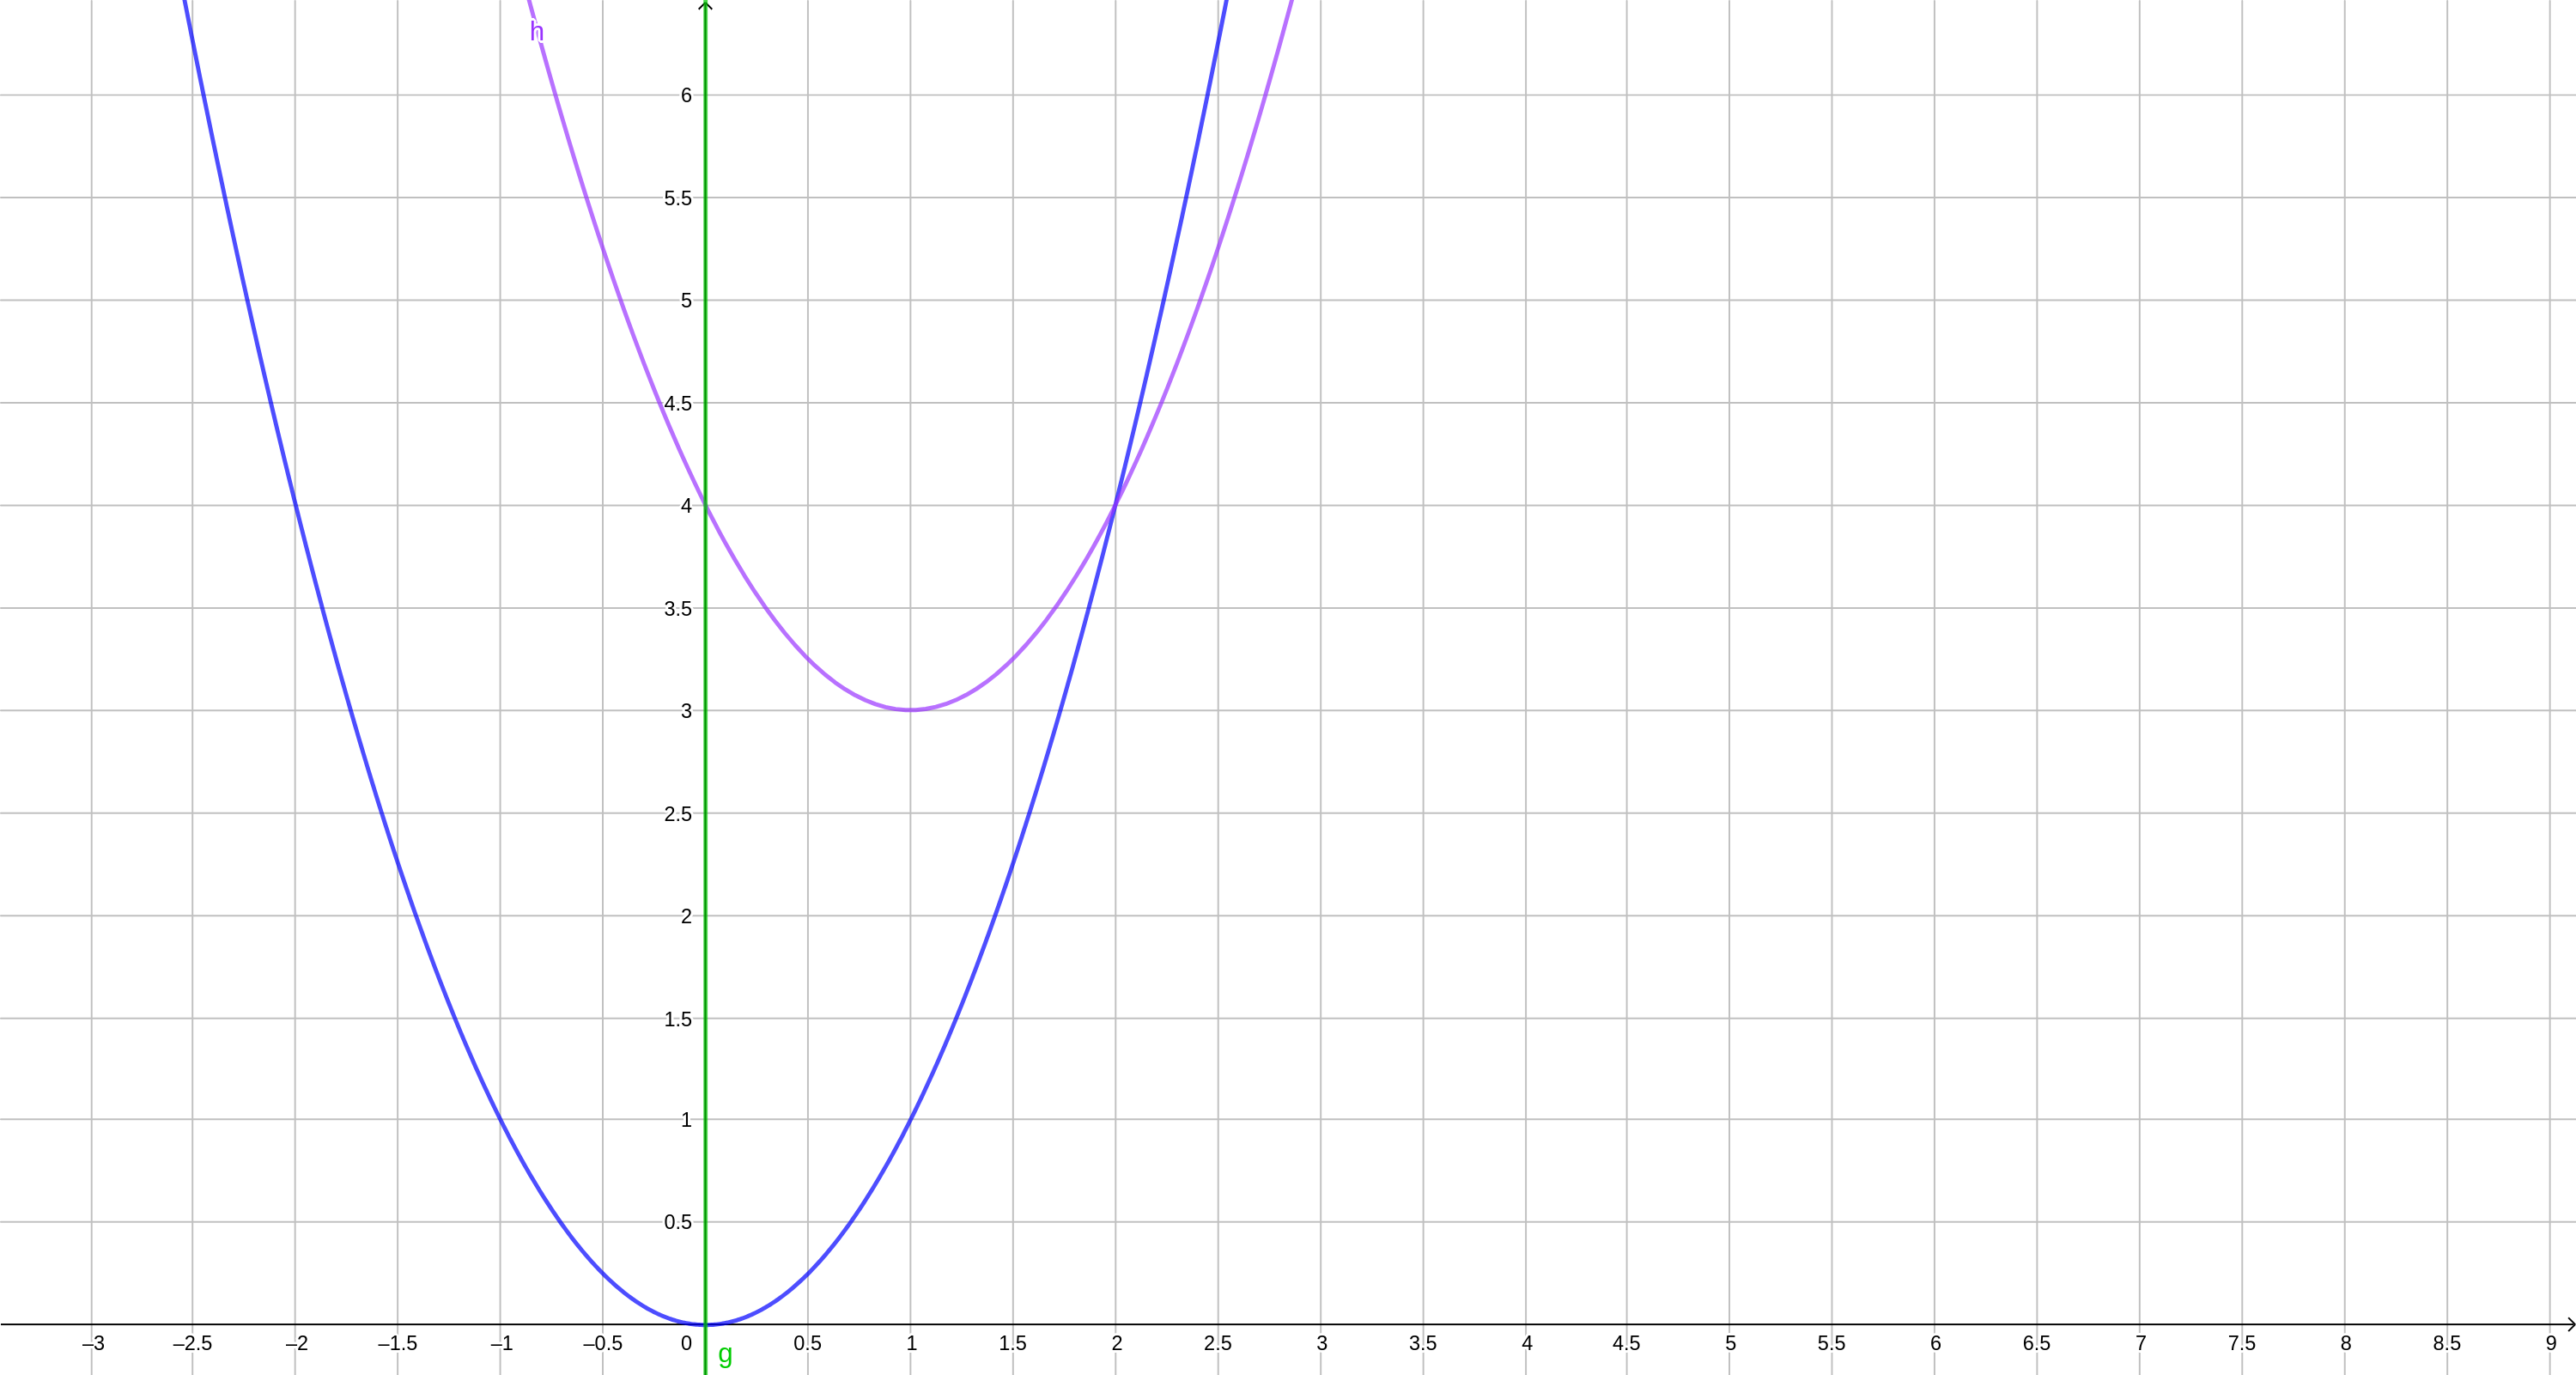
\includegraphics[width=12cm]{Parte 1/grafica5.png}
    \end{figure}
    La gráfica delimitada estará entonces en el primer cuadrante del plano cartesiano. Revisando el punto extremo dentro de las gráficas tendremos:
    \begin{align*}
        x^2 &= x^2-2x+4\\
        -2x+4 &= 0\\
        2x &= 4\\
        x &= 2
    \end{align*}
    Por lo que la operación necesaria para determinar el area de la región será determinar una integral entre $0$ y $2$, teniendo en cuenta que
    la función $g$ es mayor que la función $f$ en el intervalo dado, tendremos:
    \begin{align*}
        \int_{0}^2 g(x)-f(x)dx &= \int_{0}^2 x^2-2x+4 dx - \int_{0}^2 x^2 dx\\
        &= \int_{0}^2 x^2 dx - 2\int_{0}^2 x dx + \int_{0}^2 4 dx - \int_{0}^2 x^2 dx\\
        &= \int_{0}^2 4 dx - 2\int_{0}^2 x dx\\
        &= 8 - 2 \cdot \frac{4}{2}\\
        &= 8 - 4\\
        &= 4
    \end{align*}
    Por lo que el area de la región delimitada será $4$.
    \parte Las gráficas de $f(x) = \sqrt{x}$, el eje horizontal y la linea vertical que pasa por $(2, 0)$ \\
    \begin{figure}[h]
        \centering
        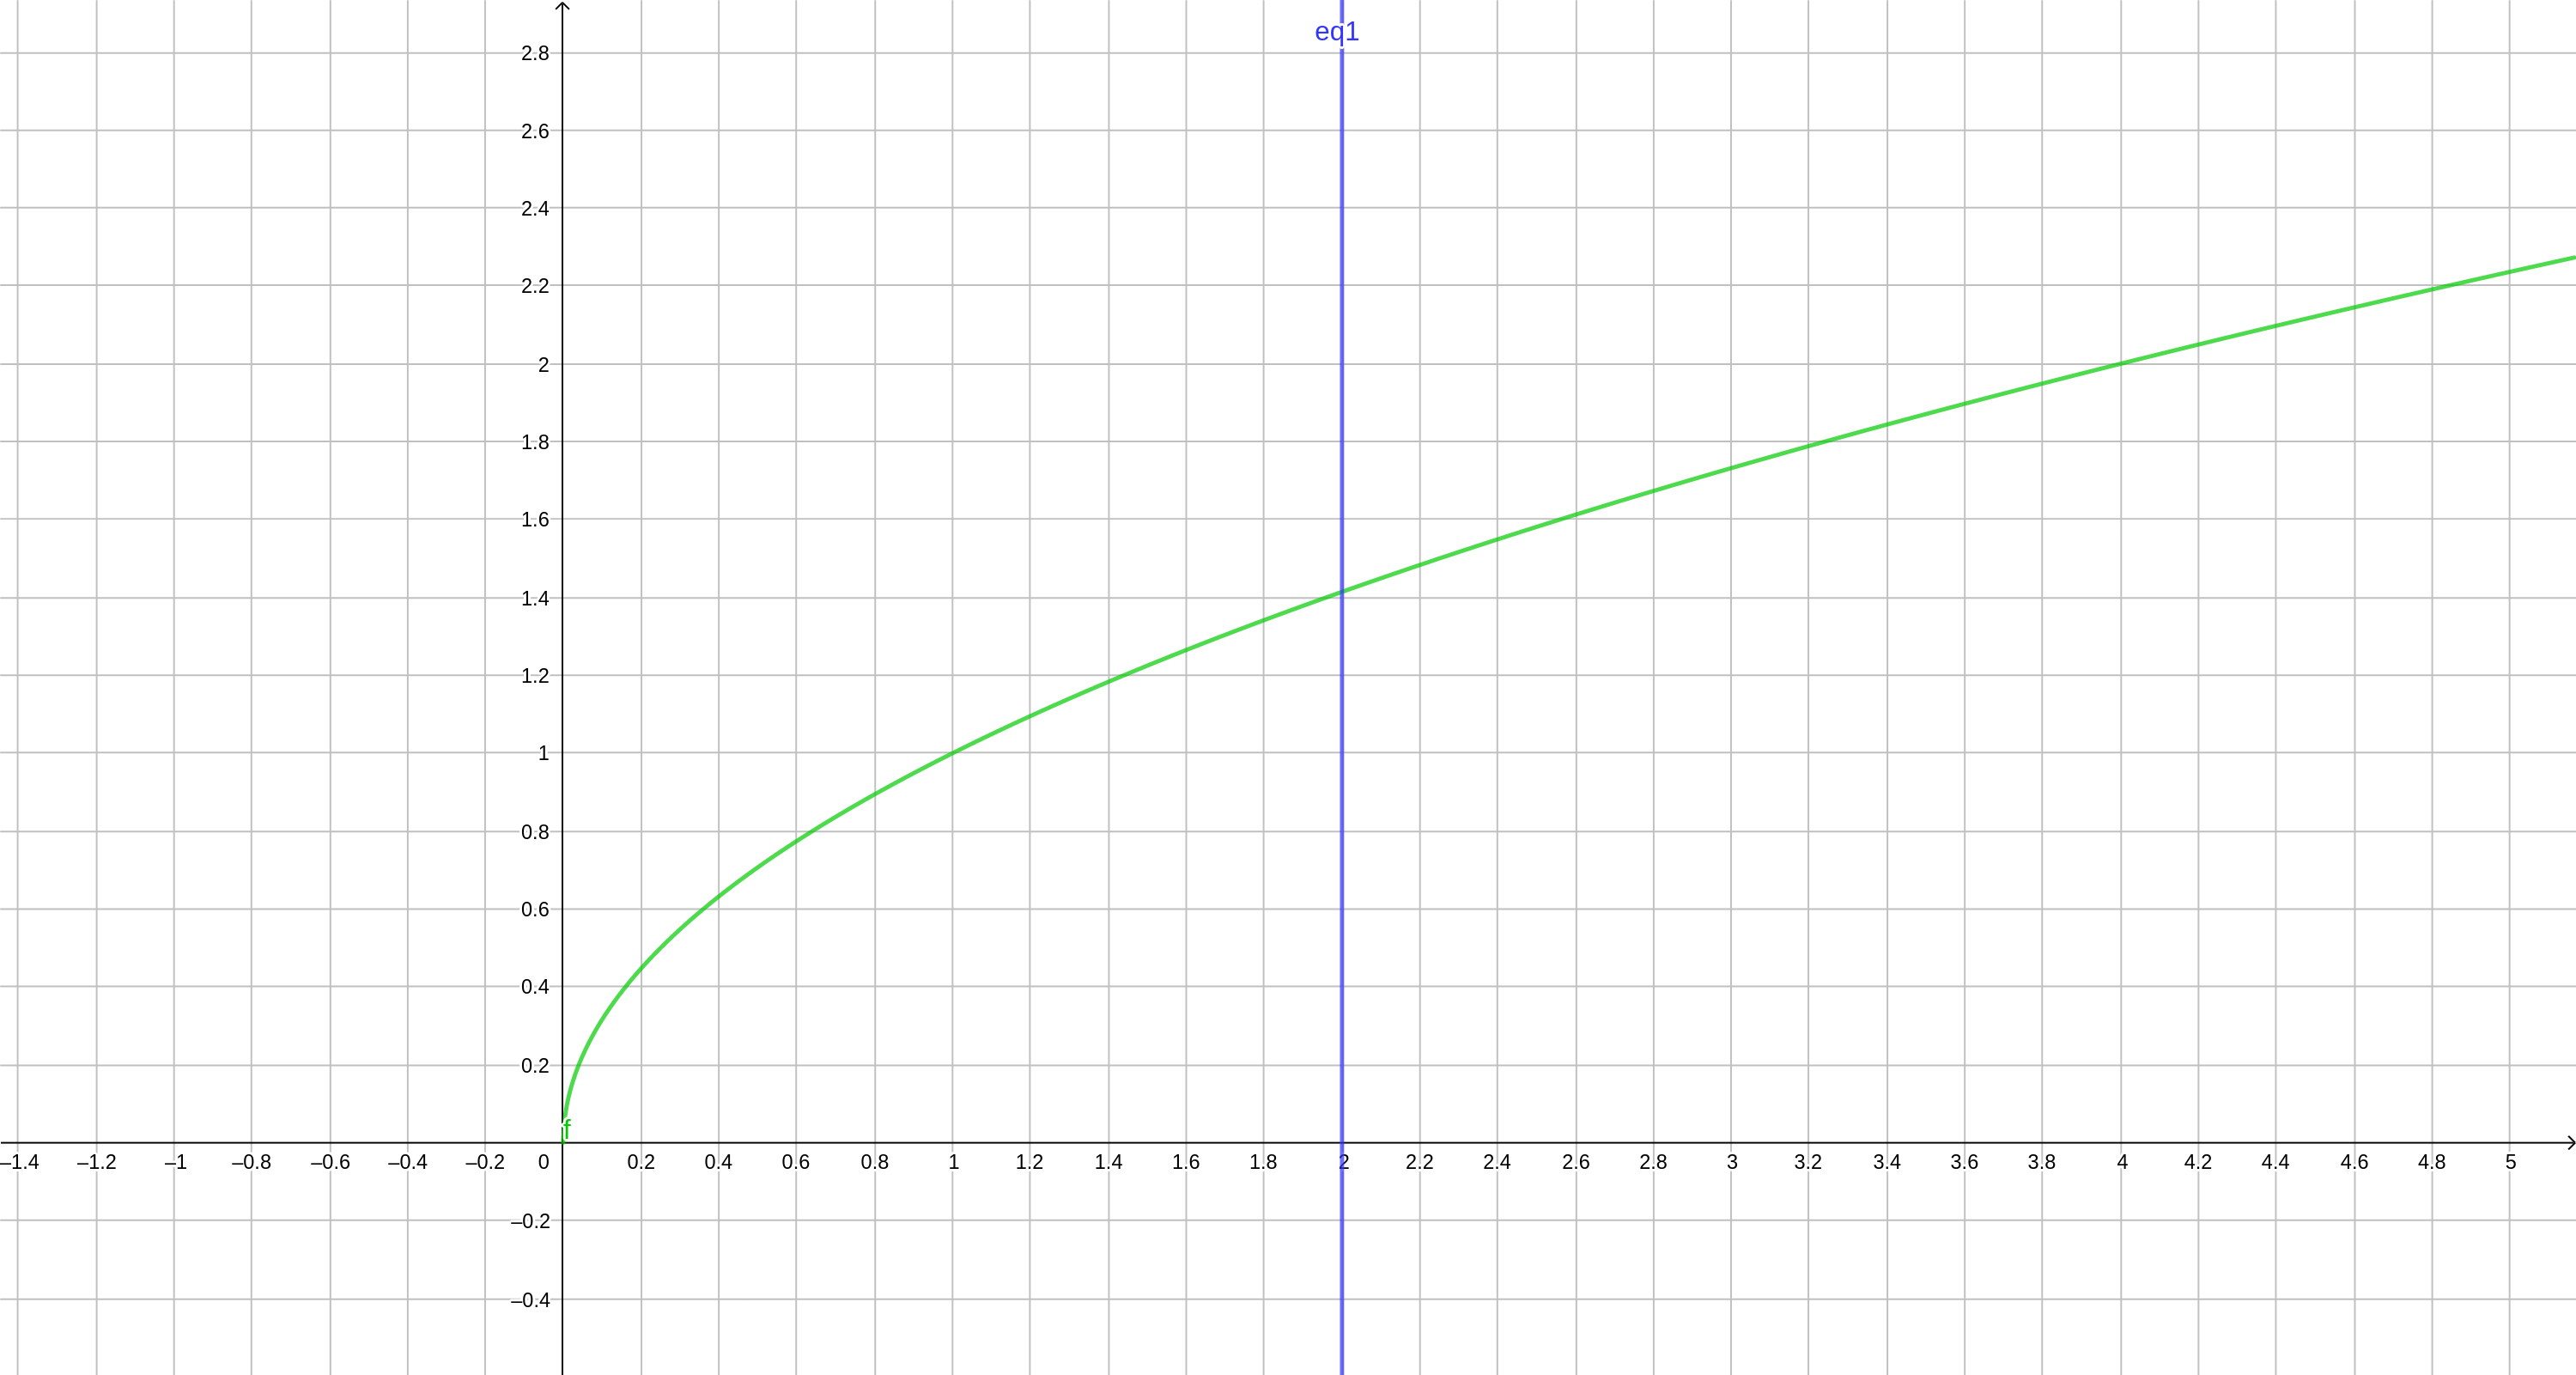
\includegraphics[width=12cm]{Parte 1/grafica6.png}
    \end{figure}
    Con el objetivo de evaluar solo integrales que sabemos determinar, tome en cuenta como referencia de eje horizontal al eje $y$.
    Luego, se puede observar que al ser gráficas "inversas" tendremos que determinar una integral entre $[0, \sqrt{2}]$. Esto será:
    \begin{align*}
        \int_{0}^{\sqrt{2}} y^2 dy &= \frac{(\sqrt{2})^3}{3}\\
        &= \frac{2\sqrt{2}}{3}
    \end{align*}
    Por lo que el area de la región solicitada será $\frac{2\sqrt{2}}{3}$. Esto de forma que la región de la función $x = y^2$ y $x=2$ en la región necesitada es
    la misma que la región de la función $y = \sqrt{x}$ y la recta $x=2$.
\end{partes}

\question \textbf{Ejercicio 9:} Determine: $$\int_{a}^b \left(\int_{c}^d f(x) g(y)\, dy\right) dx$$ en terminos de $\int_{a}^b f$ y $\int_{c}^d g$

Para empezar, es necesario notar que $f(x)$ se comporta como una constante dentro de la segunda integral, al estar en terminos de $y$. Por tanto, podemos escribir:
\begin{align*}
    \int_{a}^b \left(\int_{c}^d f(x) g(y)\, dy\right) dx &= \int_{a}^b \left(f(x) \cdot \int_{c}^d g(y) dy\right)dx
\end{align*}
Luego, con respecto a la primera integral, $\int_{c}^d g(y) dy$ se comporta como una constante, lo que permite reducir a:
\begin{align*}
    \int_{a}^b \left(f(x) \cdot \int_{c}^d g(y) dy\right)dx &= \int_{c}^d g(y) dy \cdot \int_{a}^b f(x) dx
\end{align*}
Lo que permite que la expresión original sea escrita como:
$$\int_a^b f \cdot \int_c^d g$$

\question \textbf{Ejercicio 10:} Demostrar usando la notación del Teorema 5 que:
$$m_i' + m_i'' = inf\{f(x_1) + g(x_2): t_{i-1} \le x_1, x_2 \le t_i\} \le m_i$$
\begin{proof}
    Recordando las siguientes definiciones del Teorema 5:
    \begin{align*}
        m_i' &= inf\{f(x): t_{i-1} \le x \le t_i\}\\
        m_i'' &= inf\{g(x): t_{i-1} \le x \le t_i\}\\
        m_i &= inf\{f(x)+g(x): t_{i-1} \le x \le t_i\}\\
    \end{align*}
    Primero, se demostrará que $m_i' + m_i'' = inf\{f(x_1) + g(x_2): t_{i-1} \le x_1, x_2 \le t_i\}$. Sean $x_1, x_2, x_1', x_2'$ de forma que:
    \begin{align*}
        inf\{f(x)+g(x): t_{i-1} \le x \le t_i\} &= f(x_1) + g(x_2)\\
        m_i' &= f(x_1')\\
        m_i'' &= f(x_2')\\
    \end{align*}
    Por definición es dado que:
    $$f(x_1') + g(x_2') \le f(x_1) + g(x_2)$$
    Luego, por la definción de $m_i'$ y de $m_i''$:
    \begin{align*}
        f(x_1) &\le f(x_1')\\
        g(x_2) &\le g(x_2')\\
    \end{align*}
    Lo que nos permite concluir que:
    $$f(x_1) + g(x_2) \le f(x_1') + g(x_2')$$
    Y de lo que sigue que:
    $$f(x_1) + g(x_2) = f(x_1') + g(x_2')$$
    Luego, sea $x'$ de forma que:
    \begin{align*}
        m_i &= f(x') + g(x')
    \end{align*}
    Por definición, de nuevo se tendrá que:
    \begin{align*}
        f(x_1) &\le f(x')\\
        g(x_2) &\le g(x')\\
    \end{align*}
    De lo que se concluye que:
    \begin{align*}
        f(x_1) + g(x_2) &\le f(x') + g(x')\\
        m_i' + m_i'' &\le m_i
    \end{align*}
\end{proof}

\question \textbf{Ejercicio 13:}
\begin{partes}
    \parte Demostrar que si $f$ es integrable en $[a, b]$ y $f(x) \ge 0$ para todo $x \in [a, b]$, entonces $\int_a^b f \ge 0$
    \begin{proof}
        Sea entonces $P$ una partición sobre el intervalo $[a, b]$, es notable por la hipotesis que en todo subintervalo $[x_{i-1}, x_i]$ se tendrá que
        $M_i \ge 0$ y $m_i \ge 0$. Junto con el hecho de que siempre $x_i - x_{i-1} \ge 0$ podemos concluir que para todo $i$ entre $1$ y $n$:
        \begin{align*}
            M_i \cdot (x_i - x_{i-1}) &\ge 0 & m_i \cdot (x_i - x_{i-1}) &\ge 0\\
        \end{align*}
        Por lo que en terminos más generales tendremos que:
        \begin{align*}
            \sum_{i=1}^n M_i \cdot (x_i - x_{i-1}) &\ge 0 & \sum_{i = 1}^n m_i \cdot (x_i - x_{i-1}) &\ge 0
        \end{align*}
        Por lo que $U(f)$ y $L(f)$ serán mayores o iguales a $0$ puesto que las afirmaciones anteriores se cumplen para toda partición $P$.
        Dado que $f$ es \textit{Darboux Integrable}, entonces $U(f) = L(f) = \int_a^b f$ lo que permite concluir que:
        \begin{align*}
            \int_a^b f \ge 0\\
        \end{align*}
    \end{proof}
    \parte Demostrar que si $f$ y $g$ son integrables en $[a, b]$ y que $f(x) \ge g(x)$ para todo $x \in [a, b]$ entonces $\int_a^b f \ge \int_a^b g$
    \begin{proof}
        Bajo las condiciones dadas, es de notar que $f(x) - g(x) \ge 0$ para todo $x \in [a, b]$. Luego, al ser $g$ integrable, también lo será
        $-1 \cdot g$ y al ser $f$ integrable $f-g$ es una función integrable también. Luego, gracias a la parte (a) se puede concluir que:
        \begin{align*}
            \int_a^b f-g &\ge 0\\
            \int_a^b f - \int_a^b g & \ge 0\\
            \int_a^b f & \ge \int_a^b g
        \end{align*}
    \end{proof}
\end{partes}


\question \textbf{Ejercicio 14:} Demostrar que:
$$\int_a^b f(x) dx = \int_{a+c}^{b+c} f(x-c) dx$$
\begin{proof}
    Supongase entonces que $f$ es una función integrable en $[a, b]$. Eso quiere decir que para todo $\epsilon$ mayor que $0$
    existe una partición $P_\epsilon$ de forma que:
    \begin{align*}
        U(f, P_\epsilon) - L(f, P_\epsilon) < \epsilon
    \end{align*}
    Dicha partición puede ser escrita como:
    \begin{align*}
        P_\epsilon = \{x_0, x_1, \dots, x_n\}
    \end{align*}
    Lo que permite que tomando $c \in \mathbb{R}$, para todo $i$ tal que $1\le i \le n$ se cumple que:
    \begin{align*}
        a \le x_i \le b\\
        a+c \le x_i+c \le b+c
    \end{align*}
    Por lo que $x_i+c$ pertenece al intervalo $[a+c, b+c]$ de forma que podemos definir una partición:
    \begin{align*}
        P = \{x_i + c | x_i \in P_\epsilon\}
    \end{align*}
    De manera intuitiva se define $M_i'$ y $m_i'$ de manera similar a como se haría con $M_i$ y $m_i$, y notece que todo elemento $x_j \in [a+c, b+c]$ puede ser escrito en terminos de un elemento $x_k \in [a, b]$ como $x_j = x_k + c$.
    Con eso en mente, evaularemos las sumas inferiores y superiores de $P$ sobre la función $g$ definida como $g(x) = f(x-c)$ tendremos:
    \begin{align*}
        U(g, P) &= \sum_{i =1}^n M_i' \cdot (x_i - x_{i-1}) & L(g, P) &= \sum_{i =1}^n m_i' \cdot (x_i - x_{i-1})\\
        &= \sum_{i =1}^n g(x_j) \cdot (x_i - x_{i-1}) & &= \sum_{i =1}^n g(x_j) \cdot (x_i - x_{i-1})\\
        &= \sum_{i =1}^n f(x_j-c) \cdot (x_i - x_{i-1}) & &= \sum_{i =1}^n f(x_j-c) \cdot (x_i - x_{i-1})\\
        &= \sum_{i =1}^n f((x_k +c)-c) \cdot (x_i - x_{i-1}) & &= \sum_{i =1}^n f((x_k+c)-c) \cdot (x_i - x_{i-1})\\
        &= \sum_{i =1}^n f(x_k) \cdot (x_i - x_{i-1}) & &= \sum_{i =1}^n f(x_k) \cdot (x_i - x_{i-1})\\
        &\le \sum_{i =1}^n M_i \cdot (x_i - x_{i-1}) & &\ge \sum_{i = 1}m_i (x_i-x_(i-1))\\
        &= U(f, P_\epsilon) & &= L(f, P_\epsilon)
    \end{align*}
    Lo que permite concluir la siguiente desigualdad:
    \begin{align*}
        L(f, P_\epsilon) \le L(g, P) \le U(g, P) \le U(f, P_\epsilon)
    \end{align*}
    De manera clara ya es evidente que:
    \begin{align*}
        U(g, P) - L(g, P) < \epsilon
    \end{align*}
    Por lo que $g$ es integrable sobre $[a+c, b+c]$. Note que:
    \begin{align*}
        L(f, P_\epsilon) \le L(g, P) \le \int_{a+c}^{b+c} g(x) dx \le U(g, P) \le U(f, P_\epsilon)
    \end{align*}
    Pero dado que:
    \begin{align*}
        L(f, P_\epsilon) \le \int_{a}^b f(x) dx \le U(f, P_\epsilon)
    \end{align*}
    Podemos concluir que al hacer la diferencia entre las sumas superiores y las sumas inferiores tendremos que:
    \begin{align*}
        \int_a^b f(x) dx &= \int_{a+c}^{b+c} g(x) dx\\
        \int_a^b f(x) dx &= \int_{a+c}^{b+c} f(x-c) dx
    \end{align*}
\end{proof}

\question \textbf{Ejercicio 15:} Para $a, b > 1$ demostrar que:
$$ \int_1^a \frac{1}{t} dt + \int_1^b \frac{1}{t} dt = \int_1^{ab} \frac{1}{t} dt$$
\begin{proof}
    Gracias al hecho de que:
    \begin{align*}
        \int_a^1 \frac{1}{t} dt &= \int_b^{ab} \frac{1}{t} dt
    \end{align*}
    La expresión original puede ser escrita como:
    \begin{align*}
        \int_1^a \frac{1}{t} dt + \int_1^b \frac{1}{t} dt  &= \int_b^{ab} \frac{1}{t} dt + \int_1^b \frac{1}{t} dt\\
        &= \int_1^b \frac{1}{t} dt + \int_b^{ab} \frac{1}{t} dt\\
        &= \int_1^{ab} \frac{1}{t} dt
    \end{align*}
\end{proof}

\question \textbf{Ejercicio 20:} Suponga que $f$ es una función no decreciente en $[a, b]$. 
\begin{partes}
    \parte Si $P = \{t_0, \dots, t_n\}$ es una partición de $[a, b]$. ¿Que es $U(f, P)$ y $L(f, P)$?\\
    Gracias a ser no decreciente, se tendrá que:
    \begin{align*}
        U(f, P) &= \sum_{i=1}^n M_i(x_i - x_{i-1}) & L(f, P) &= \sum_{i=1}^n m_i (x_i - x_{i-1})\\
        &= \sum_{i=1}^n f(x_i)(x_i - x_{i-1}) & &= \sum_{i=1}^n f(x_{i-1})(x_i-x_{i-1})
    \end{align*}
    En terminos un poco más explicitos, $U(f, P)$ será la suma de areas de los rectángulos cuyas alturas son
    $f(t_1), f(t_2), \dots, f(t_n)$ y $L(f, P)$ serála suma de areas de los rectángulos cuyas alturas son 
    $f(t_0), f(t_1), \dots, f(t_{n-1})$.
    \parte Suponga que $t_i - t_{i-1} = \delta$ para todo $i$. Demostrar que $U(f, P) - L(f, P) = \delta[f(b)-f(a)]$
    \begin{proof}
        Sea $f$ una función no decreciente en $[a, b]$ y una partición $P$ de forma que $t_i - t_{i-1} = \delta$ para todo $i$ entre $1$ y $n$.
        Entonces:
        \begin{align*}
            U(f, P) - L(f, P) &= \sum_{i = 1}^n M_i (t_i - t_{i-1}) - \sum_{i = 1}^n m_i(t_i - t_{i-1})\\
            &= \sum_{i = 1}^n (M_i - m_i)(t_i - t_{i-1})\\
            &= \sum_{i = 1}^n (f(t_i) - f(t_{i-1}))(t_i - t_{i-1})\\    
            &= \sum_{i = 1}^n (f(t_i) - f(t_{i-1})) \delta\\    
        \end{align*} 
        \begin{align*}
            &= \delta \sum_{i = 1}^n (f(t_i) - f(t_{i-1}))\\    
            &= \delta [f(t_n)-f(t_0)]\\ 
            &= \delta [f(b)-f(a)]\\   
        \end{align*}
    \end{proof}
    \parte Demostrar que $f$ es integrable
    \begin{proof}
        Sea $f$ una función no decreciente en $[a, b]$. Tome $\epsilon > 0$, definamos entonces $P_\epsilon = {x_0, x_1, \dots, x_n}$ para $n > \frac{(b-a)(f(b)-f(a))}{\epsilon}$ y de forma que
        $t_i - t_{i-1} = \frac{(b-a)}{n}$ .Se tendrá entonces:
        \begin{align*}
            U(f, P) - L(f, P) &= \sum_{i = 1}^n M_i (t_i - t_{i-1}) - \sum_{i = 1}^n m_i(t_i - t_{i-1})\\
            &= \sum_{i = 1}^n (M_i - m_i)(t_i - t_{i-1})\\
            &= \sum_{i = 1}^n (f(x_i) - f(x_{i-1}))(\frac{b-a}{n})\\
            &= \frac{b-a}{n} \cdot \sum_{i = 1}^n (f(x_i) - f(x_{i-1}))\\
            &= \frac{b-a}{n} \cdot (f(b)-f(a))\\
            &= \frac{(f(b)-f(a))(b-a)}{n}\\
            &\le \epsilon
        \end{align*}
        Y dado que la diferencia entre las sumas superiores e inferiores es menor que $\epsilon$ para todo $\epsilon > 0$,
        entonces $f$ es \textit{Darboux Integrable}. 
    \end{proof}
    \parte Dar un ejemplo de una función no descreciente en $[0, 1]$ que sea discontinua en infinitos puntos.\\
    Definase el siguiente conjunto $F$:
    \begin{align*}
        F := \left\{ \frac{1}{n} \in \mathbb{R} | n \in \mathbb{N} \right\}
    \end{align*} 
    Entonces defina la función $f: \mathbb{R} \setminus F \to \mathbb{R}$ de forma que $f(x) = x$. Es evidente que la función es
    no decreciente y además posee una infinidad de discontinuidades.
\end{partes}
\end{document}